\documentclass[10pt]{article}
\usepackage[margin=0.6in]{geometry}
\usepackage{graphicx}
\usepackage{booktabs}
\usepackage[hidelinks]{hyperref}
\usepackage{enumitem}
\setlist{nosep,leftmargin=1.2em}
\setlength{\parindent}{0pt}
\setlength{\parskip}{3pt}
\pagestyle{empty}
\begin{document}

{\large\textbf{TOI-913 (TIC 407126408): a 5.45-day, 1.1\,$R_\oplus$ transit candidate}}\\
\small Josh Gold, independent researcher, Acton, MA. One-page summary, 16 October 2026. Not peer reviewed.
Preprint (version 2): \href{https://doi.org/10.5281/zenodo.23415929}{doi:10.5281/zenodo.23415929}.
Code: \href{https://github.com/killercatfish/tess-hunt}{github.com/killercatfish/tess-hunt}.
\normalsize

\textbf{The signal.} $P = 5.450138 \pm 0.000016$\,d, depth $196^{+24}_{-21}$\,ppm, duration 2.4\,h, $R_p = 1.12 \pm 0.09\,R_\oplus$ if on the target
(K dwarf, $V=10.5$, 65\,pc, Dec $-80.8^\circ$). 34 transits in SPOC 2-min data, Sectors 12--102. Inside TOI-913\,b ($P_b/P = 2.037$).
\textbf{Not first:} the open-source \texttt{eumemic/exoplanets} search detected it on 2026 Oct 8 (MES 8.0, below its candidate cut of 10).
Ours is an independent detection plus vetting.

\begin{center}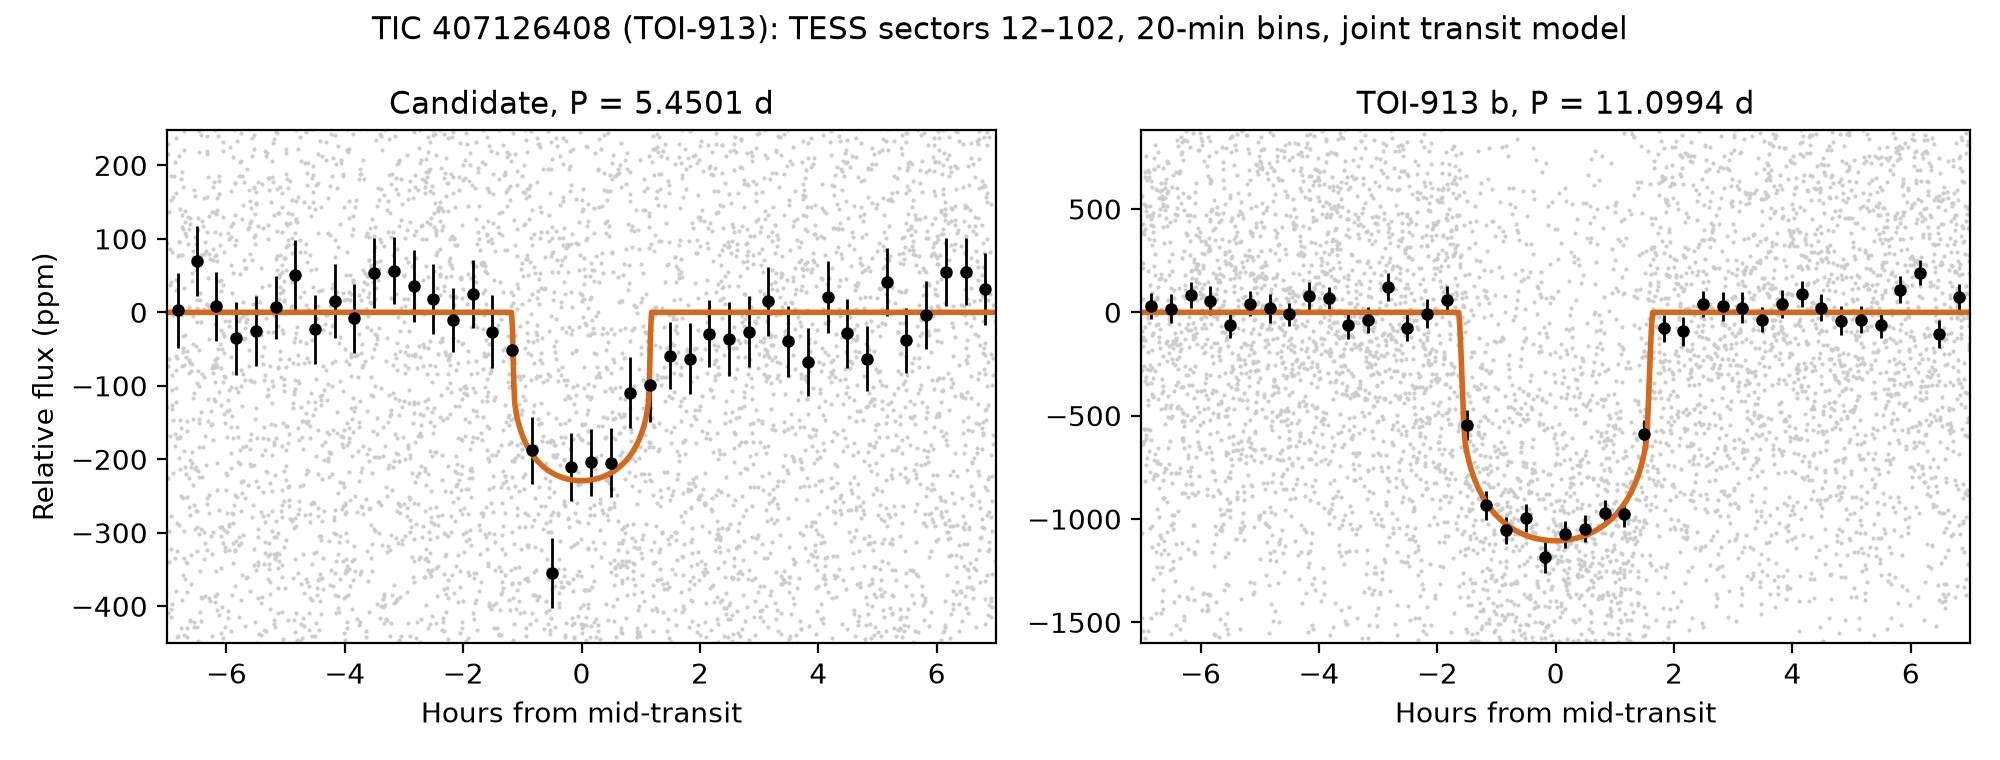
\includegraphics[width=0.82\textwidth]{../figures/fig1_fold.png}\end{center}

\begin{minipage}[t]{0.49\textwidth}
\textbf{What it survives}
\begin{itemize}
\item Nine of ten automated tests (odd/even $0.7\sigma$; no secondary; size; harmonic; per-sector; injection); shape test inconclusive.
\item Season holdout: 3 of 4 hidden seasons show the transit at $>2\sigma$ (the fourth $1.8\sigma$).
\item Recovered as the strongest periodic signal in QLP FFI photometry.
\item Empirical FAP $<1.5\%$ (200 block-shuffled light curves). Inverted light curve: strongest unrelated peak SDE 14.5 vs 21.7.
\item Free-density fit $2.43^{+0.97}_{-1.01}\,\rho_\odot$ vs catalogue $2.09 \pm 0.45$.
\item Not a 5:1 harmonic of a 27.3\,d systematic (drifts 0.59 of a period).
\item TRICERATOPS with Zorro speckle, a galaxy removed: FPP 0.036, NFPP 0.023. \textbf{Neither validated nor ``likely planet''} (both need NFPP $<0.001$).
\end{itemize}
\end{minipage}\hfill
\begin{minipage}[t]{0.49\textwidth}
\textbf{What is weak or not done}
\begin{itemize}
\item \textbf{9.5$''$ background giant} (TIC 407126405, needs a 1.1\% eclipse): excluded only by transit duration from its TIC radius. Centroids cannot separate it (ours $p=0.44$; eumemic's $0.62$).
\item \textbf{26.5$''$ star} (TIC 407126406, $T=17.0$, needs a 23\% eclipse): carries most of the NFPP. Our injection-calibrated per-sector centroids only weakly disfavour it ($p=0.02$; 0.21 at 150\,ppm), as of 16 Oct, after version 2. The 58$''$ star is rejected ($p<5\times10^{-6}$).
\item Single-transit depths scatter somewhat more than their errors ($\chi^2/\mathrm{dof}=1.51$; 21\% of off-transit phases as large).
\item Pipeline recall: it missed 7 of 17 of eumemic's signals in a blind re-vet (stops at the first sub-threshold peak). Validation: 23 of 26 known planets at the right period, 8 of 9 EBs rejected, tuned on the same set.
\item Built with substantial AI assistance (Claude), directed by me. I checked the key numbers by hand and every number in the preprint against its result file. No professional astronomer has checked it.
\end{itemize}
\end{minipage}

\textbf{Next tests.} (1) Seeing-limited photometry of TIC 407126406 (and the giant) during a predicted transit; the star is at Dec $-81^\circ$, so this needs a southern telescope; ephemeris good to $\pm15$\,min in late 2026.
(2) TESS Sector 114 (Feb--Mar 2027): transit times pre-registered before the data exist (\href{https://doi.org/10.5281/zenodo.23290795}{doi:10.5281/zenodo.23290795}); result published within 30 days whatever it shows.

\small Inspired by P.~Rabtsevich's single-star TESS method (\href{https://doi.org/10.5281/zenodo.22967456}{doi:10.5281/zenodo.22967456}).
\end{document}
